\section{Explored File Formats}

The following file formats have been explored to create Polyglot files.

\begin{itemize}
  \item WASM - Requires offset at byte 0
  \item ZIP -  Doesn't required offset at byte 0
  \item PNG - Requires offset at byte 0
  \item JPEG - Required offset at byte 0
  \item PDF - Doesn't required offset at byte 0
  \item GIF - Requires offset at byte 0
  \item ISO - Doesn't required offset at byte 0
  \item NES - Requires offset at byte 0
\end{itemize}

We'll now describe how each of them works and how can we make use of the format specification to hide other
files within it. We won't go deeply into the details just enough so that we can create Polyglot Files.

\subsection{PDF}
The PDF specification is very verbose and long over 700 pages \cite{PDF}. We don't need to
go through the whole specification in order to make use of its features for our benenfit. The following image  
describes a minimal PDF that has the core components of a PDF.

\begin{figure}[h]
    \center
    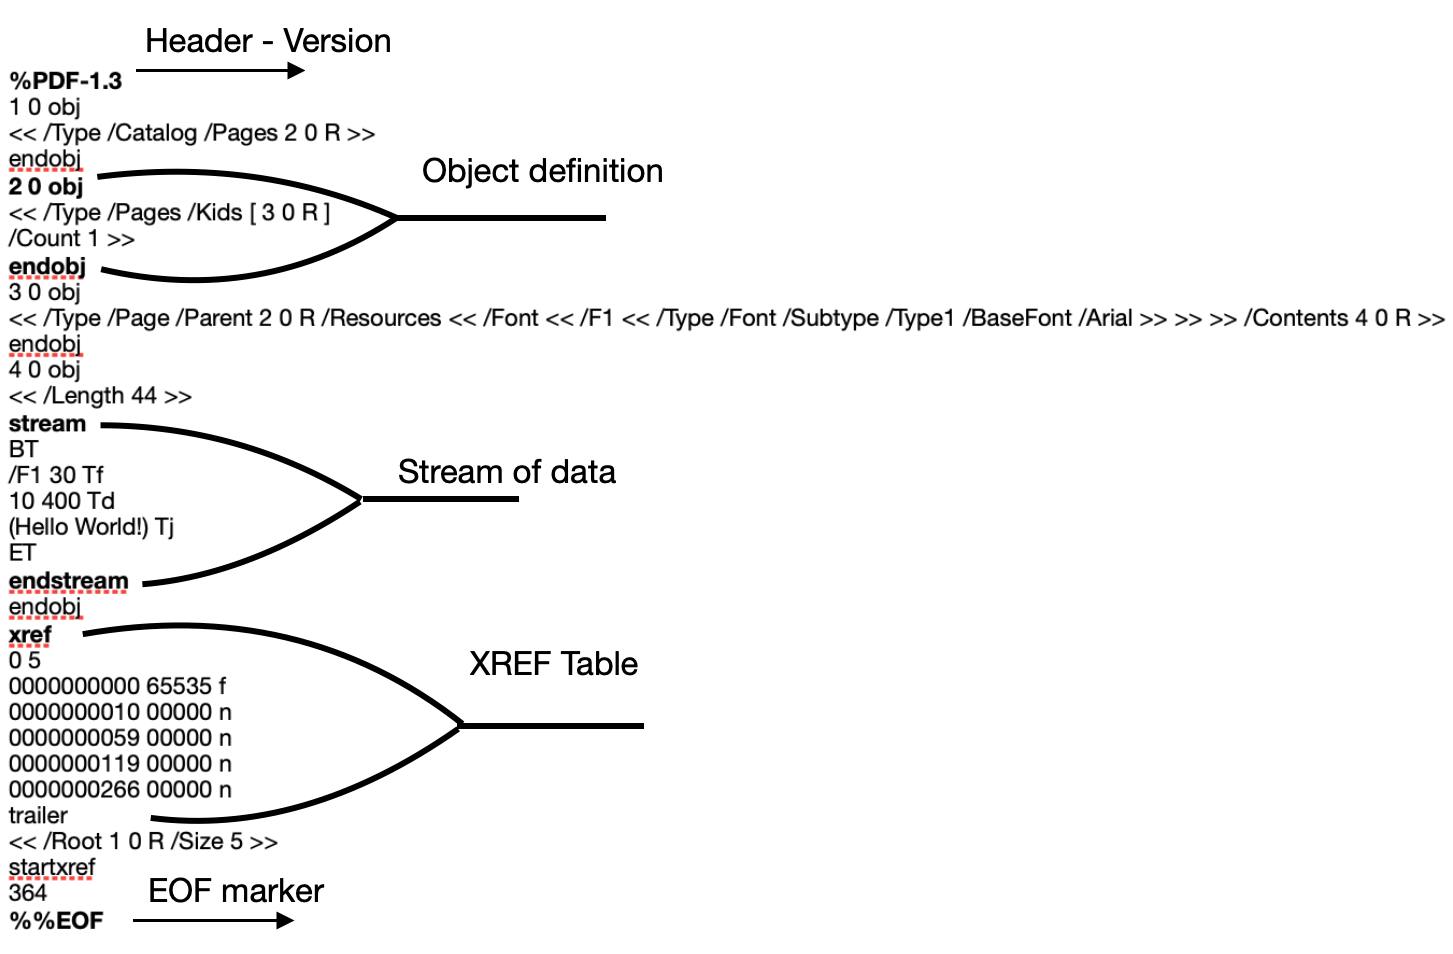
\includegraphics[width=17cm]{images/pdf.png}
    \caption{minimal PDF}
\end{figure}

A PDF is made up of objects that are referenced in the XREF table that is present at the end of the PDF, if it's there, there is not requirment on having
the XREF table. The XREF table contains the offset, of each of the defined objects, in bytes from the start of the file. An object
has definition for Fonts, Page layout, contents etc... We don't need to get to deep into this what we only care about the \textbf{Stream} part within the object.

A \textbf{Stream} is an arbitrary sequence of bytes of any length, that could be encoded/decoded or compressed \cite{PDF-Stream}. The key word for us is that it can
contain any data of any length. This is exactly what we need to create Polyglots files. Anything can be hidden within a stream in a PDF.

In the specification of PDF it actually states that the header offset is required at offset 0, however. In practice this is not the rule but rather the exception.
Thus PDF files can be mixed with other file formats that require offset at 0.

\subsection{ZIP}

ZIP is the second format that doesn't require offset at byte 0. This is purely due to historical reasons that was to minimize the number of floppy disks swaps as writing to disks
was at that time when the specification was created very time consuming. ZIP are actually parsed bottom-up. To have a valid ZIP file we need to have a \textbf{Central Directory}
that contains the name of the files with metadata and offsets that are relative to the central directory \cite{zip}.

\begin{figure}[h]
    \center
    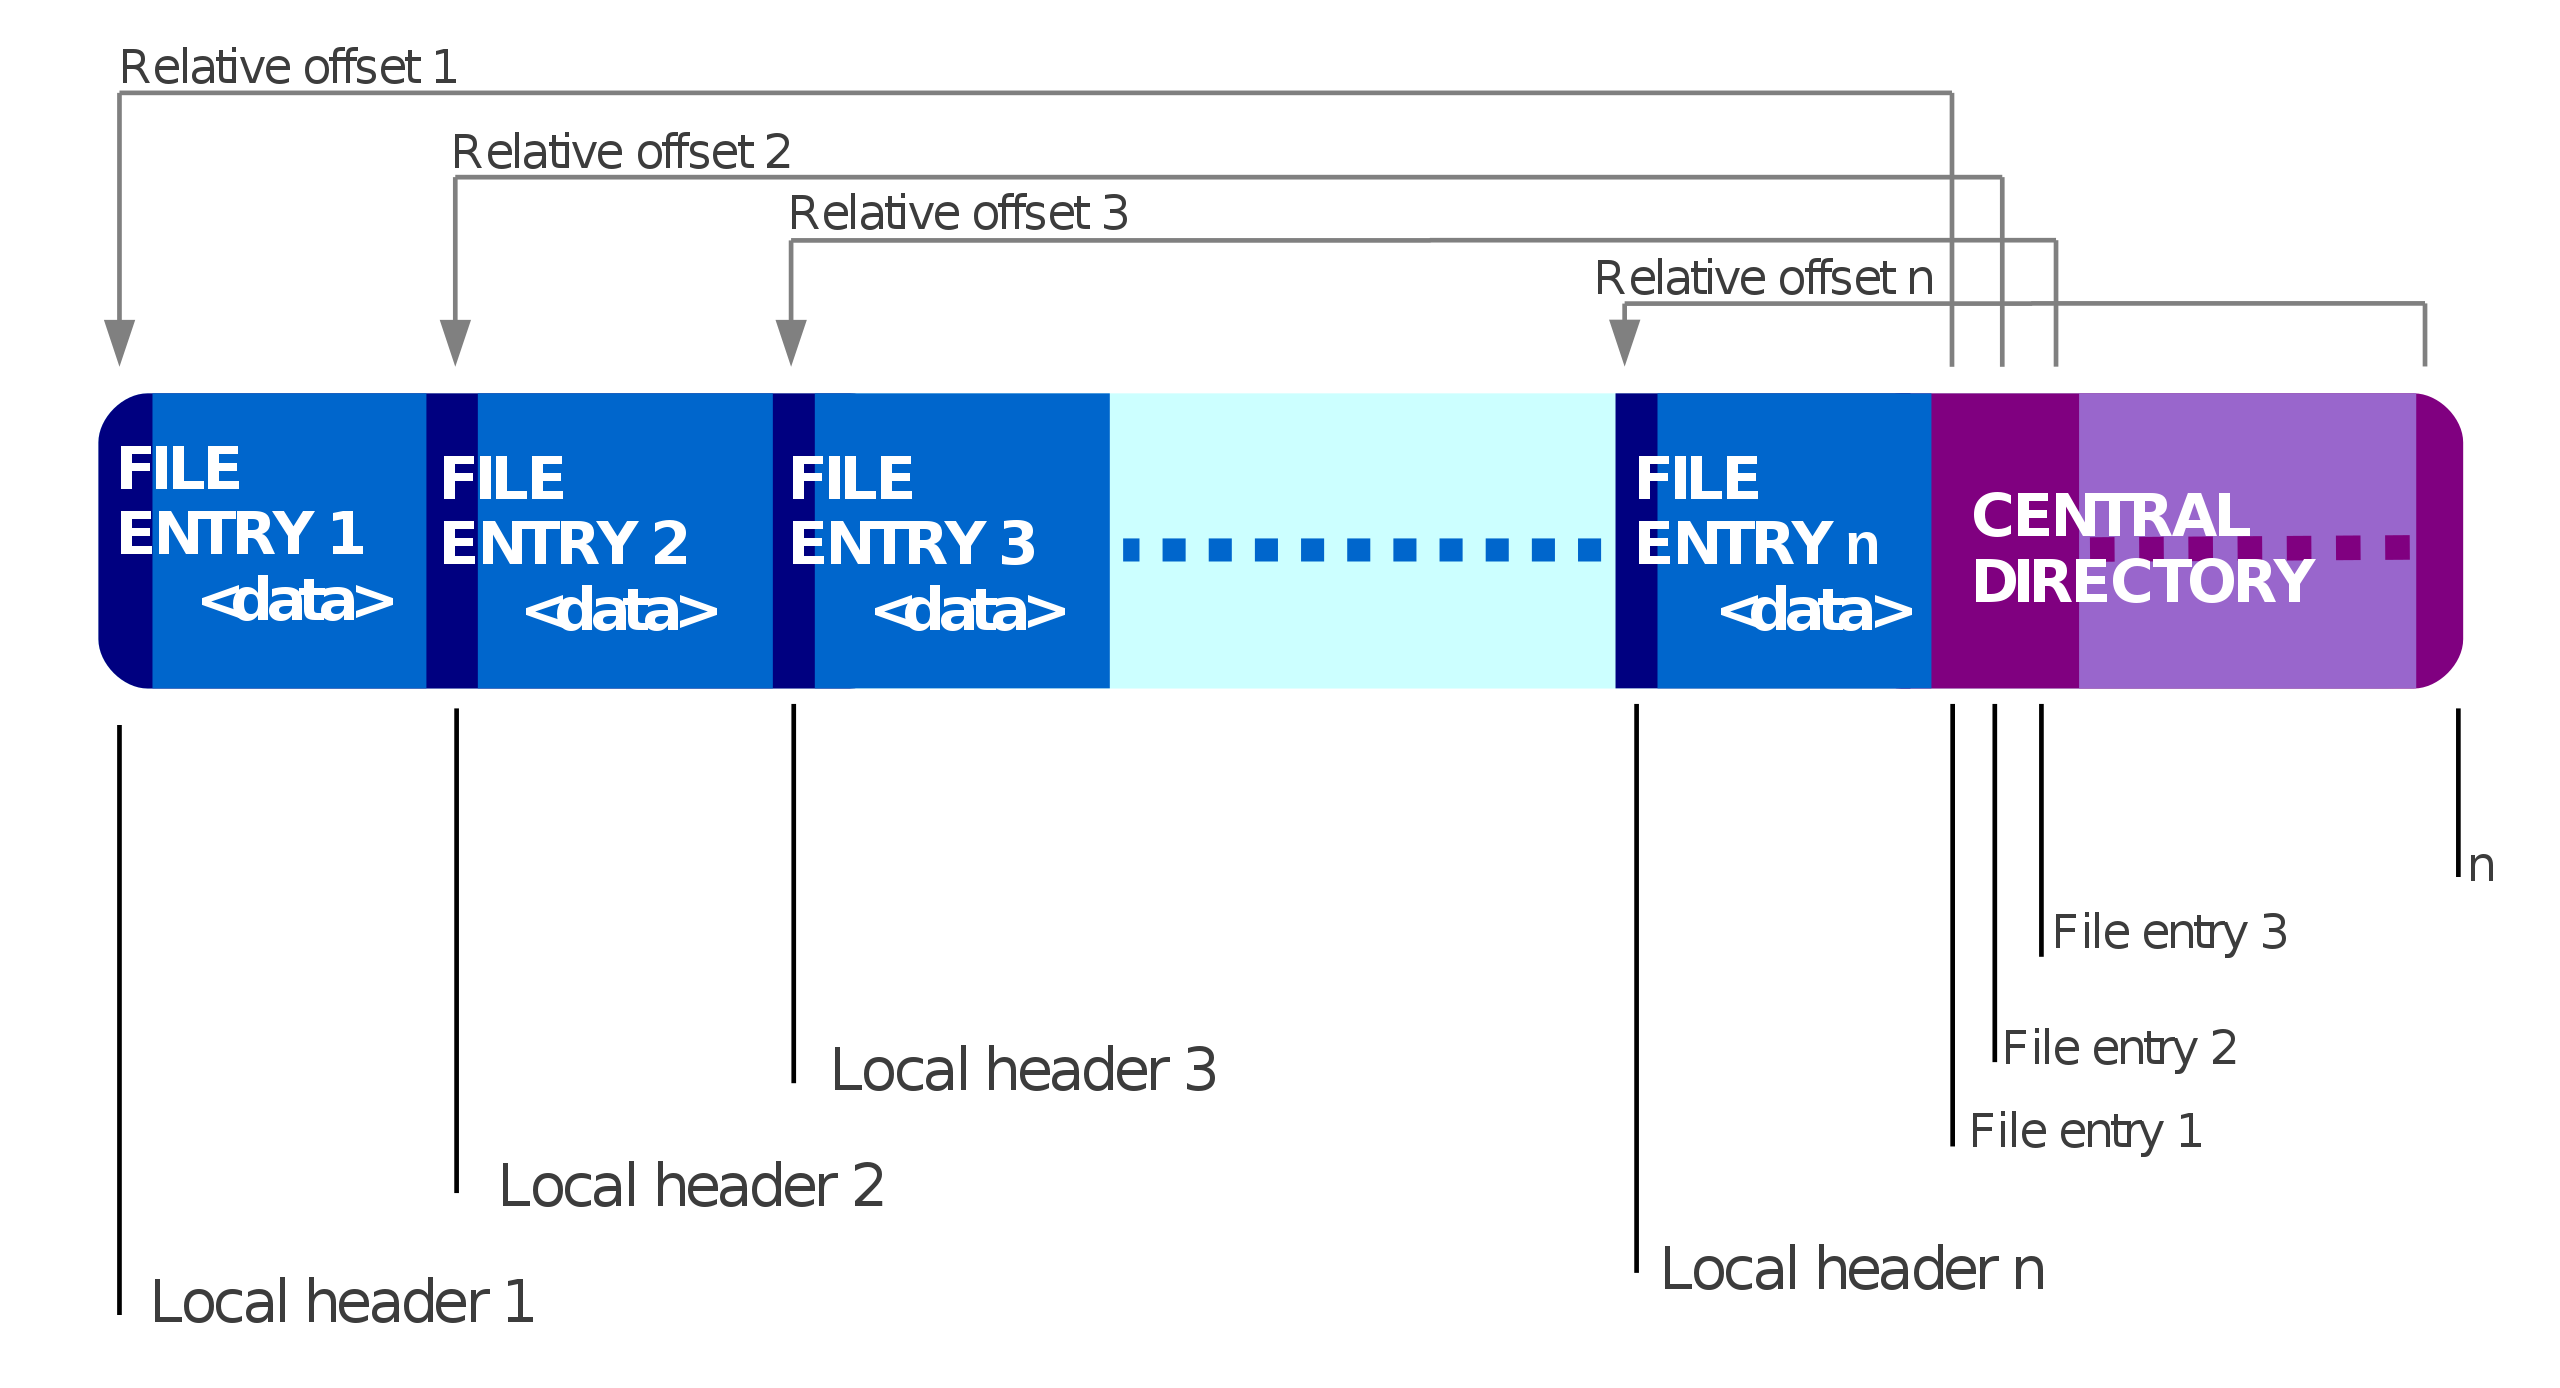
\includegraphics[width=8cm]{images/zip.png}
    \caption{ZIP Layout\cite{zip}}
\end{figure}

Each entry that the central directory refers to starts with a \textbf{Local File Header} that contains the size, name, comments etc. Followed by this is the compressed/uncompressed encrypted/un-encrypted data.

There are two ways for creating Polyglots with ZIP files, injecting ZIP within other files such as PDF, or inject other files into the ZIP.

For the former option you would expect that the \textbf{Central Directory} needs to be the last sequence of bytes in the file. This is not the case,
it can be at any position, as long as it's not too far from the end of it as in this case the parsers would give up finding the central directory.
There exists a workaround that would allow to have the the ZIP at any location by just making a copy of the central directory and storing it somewhere near the end \cite{Ange3}.

The latter makes use of the uncompress/un-encrypted data, just storing the raw file within the archive.


\subsection{PNG}

A PNG starts with the magic number followed by a sequence of chunks and an EOF chunk.
The individual chunks describe its contents. There are two types of chunks critical and anciliary. Critical chunks always start with a capital letters, whereas anciliary start with lower-case letters.
The layout of a single chunk is constructed by concatinating the following pieces, the length of the chunk, type identifier, the data itself and the crc32 checksum of the whole chunk.

The first chunk following after the magic number must be the IHDR chunk which contains information about the encoded image. After any chunk sequence can follow. The data for the image is encoded in IDAT chunks.

A minimal PNG is visualized in the following figure.

\begin{figure}[h]
    \center
    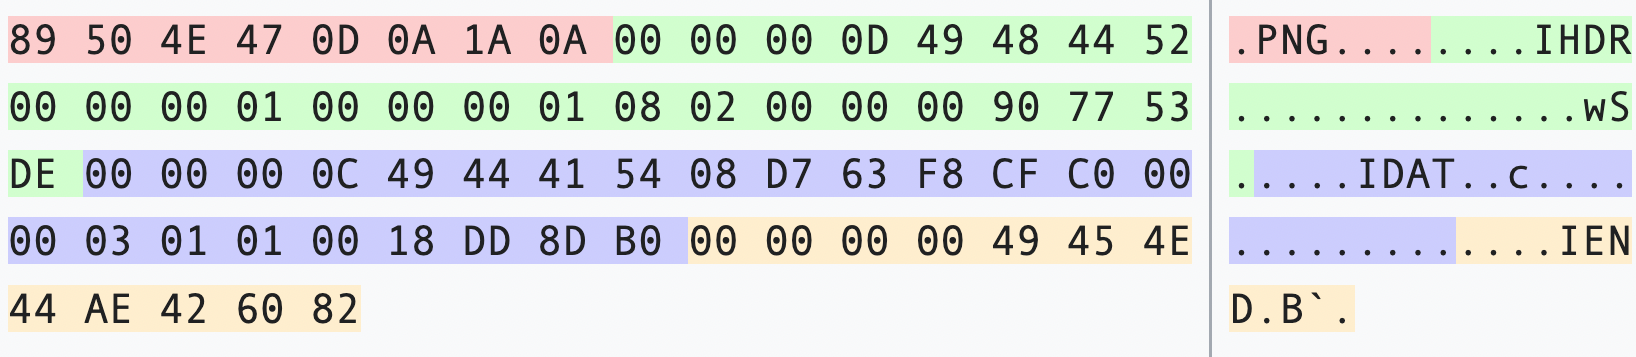
\includegraphics[width=8cm]{images/png.png}
    \caption{PNG Layout\cite{png}}
\end{figure}

To create a Polyglot file we make use of the anciliary chunks. When a PNG decoder encounters an anciliary chunk that it doesn't
recognize it can safely skip over it and continue reading the image data. We can make use of this to hide other files within a PNG
file format. Interestingly we can even make up our own chunk identifier as the decoder with just ignore it, names such as $aaaa$ or $bbbb$
are valid.



\subsection{JPEG}

JPEG a bit more complicated compared to PNG but it uses very similar concepts. JPEG start with a magic number followed by segments and ends with an
EOF marker segment. The layout of the segment is actually very different from PNGs. A segment is recognized by enclosing the data with marker bytes. The
more common segments are listed in the table to the right.

\begin{figure}[h]
    \center
    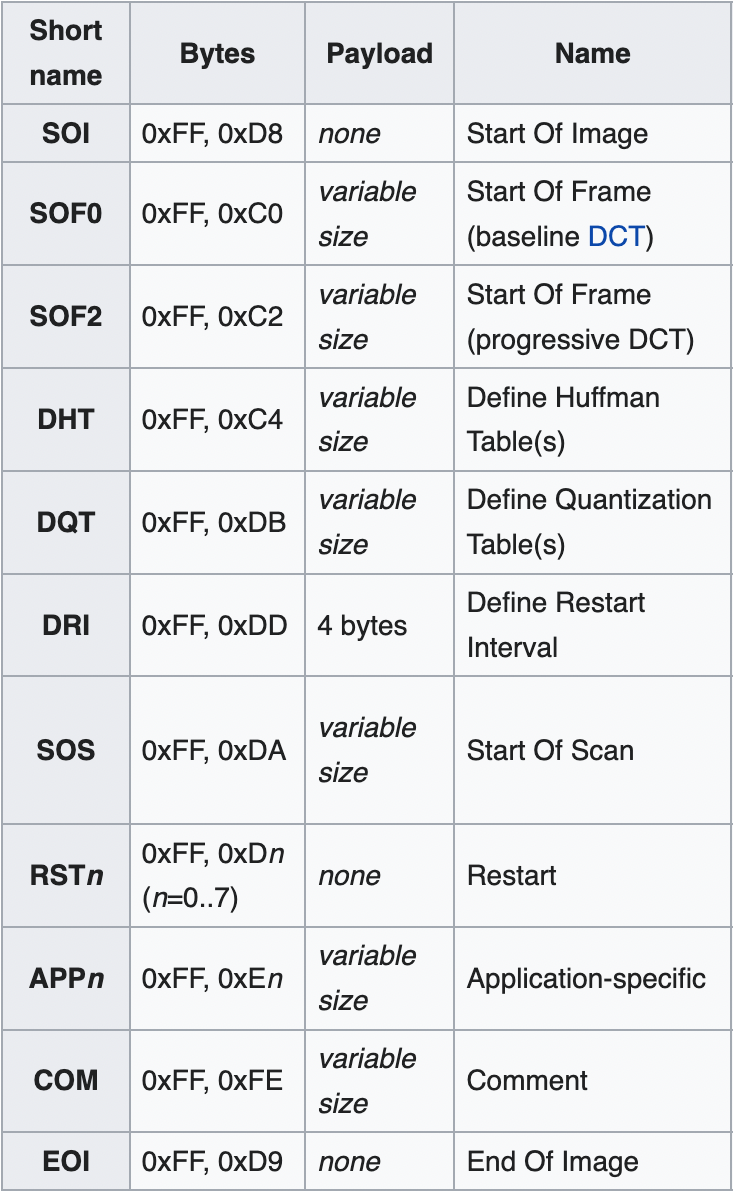
\includegraphics[width=7cm]{images/jpeg.png}
    \caption{JPEG segments\cite{jpeg}}
\end{figure}

To create a Polyglot File we simply make use of the comment segment, similarly as with PNG, and enclose our data within the \textbf{xFF xFE} bytes.

\subsection{GIF}

GIF is another image format which we can use to hide other files in. The pattern is same, there is a Header, data describing the
GIF and an EOF marker. Without going much into the details here there also is a comment section in GIF that allows us to store arbitrary
data. The catch here is that it's limited in size. The maximum amount of data a comment can store is 255 bytes \cite{gif}

The comment section in the GIF can be inserted between any two segments however the start of it has to be strictly after the Header, logical screen descriptor and the global color table,
if there is one present. The comment section is denoted by bytes \textbf{$0x21$, $0xFE$}, followed by the length of the data, the data itself and terminated with \textbf{$0x0$}

\subsection{MP3}

The MP3 file format doesn't have something simlar to comments, it however can be used in conjuction with ID3 metadata container. ID3 is used for information
such as the artist name, album etc. What's interesting for us with this is that this metadata container has support for comments section. There are two version
for ID3, v1 and v2 both can be present for a single mp3 file. Version 1 is roughly 127 bytes long and is always the last 127 bytes of the MP3 file. For version 2
the position is at the start of the MP3 file and there are no limits regarding the size\cite{mp3}.

To create a Polyglot file we need to add a comment section for the ID3v2 metadata. The comment section layout structure is made up out of the encoding, language
description and text as depicted by the following snippet which is a high-level description.

\begin{verbatim}
id3v2.CommentFrame{
     Encoding:    id3v2.EncodingUTF8,
     Language:    "eng",
     Description: "eng",
     Text:        hidden_file_bytes,
}
\end{verbatim}

for our use-case the values of the language or description doesn't matter nor the encoding we only care about the data we can hid inside the comment section.

\subsection{WASM}

WASM is a very recent format that was released in 2017 and actually has some standardization, yet we can still use the specification for our benefit.
WASM starts with a Header $0asm$ and 4 bytes for a version number of the binary, after wihch an arbitrary sequence of sections can follow. Each section has its
own identification code ranging from 0 to 11. A section layout is made out of the identification code, the length of the section encoded using LEB128 and
the data for the section itself. One particular section is intersting and that is the custom section that's identified with 0x0\cite{wasm}.

This section can be used for storing arbitrary information. For us this means that we can create Polyglot files by storing other files inside the custom sections
the length of the custom section is variable in size as long as the size doesn't exceeds WASM uint32 which is 4 bytes, giving us a lot more freedom of in terms
of the hidden data.

\subsection{ISO}

ISO format is very different from all of the just mentioned formats. ISO is a disk image that contains all the necessary things that would be needed when written to an optical disk. There are no comments or metadata that we can make use of. There also is no Header that's required at offset 0 nor a EOF marker, however.
There is a magic number that is present at byte 32769 \cite{iso}.

We can use unused zero-fill memory to create polyglot files from ISO formats, as described in Section 3.2 for cavities.
Since the magic number is placed at position 32kb there usually is some unused space
at the beginning that we can make use of; this is also true for the end of the ISO format. 
Unfortunutely I couldn't find a pattern that would always work and just tried this with trial and error until it worked.

\subsection{NES}

For NES ROM files there are no comments/metadata either so the only way to create a Polyglot is using cavities i.e. directly injected the file into padded/unused static memory
or we can use a Trainer that is part of the NES ROM. Trainer is 512 bytes of memory that most games do not use and it was sometimes used to inject cheat codes. For our purpose
we could use this to store other files that are smaller than 512 bytes \cite{nes}. This is a bit harder to do as most emulators that I've tried didn't accept trainers as valid
but it's still an option that exists. Trainer follows directly after the Header.

\begin{verbatim}
Header (16 bytes)
Trainer, if present (0 or 512 bytes)
...
\end{verbatim}

To enable the Trainer we need to set the 3rd bit of the 6th byte from the header and then we need to add 512 bytes, if there not present yet, directly following after
the header.
